\chapter{Background}
\label{chapter:background}
%TODO: Add pretty pictures from other people's great

DHTs have been a vibrant area of research for the past decade, with several of the concepts dating further back.
Numerous DHTs have been developed over the years.
This is partly because the process of designing DHTs involves making tradeoffs, with no choice being strictly better than any other.

\section{What is a Distributed Hash Table?}


\subsection{Terminology}
% % %unified terminology
The large number of DHTs have lead many papers use different terms to describe congruent elements of DHTs, as some terms may make sense only in one context.
Since this paper will cover multiple DHTs that would use different terms,  we have created a unified terminology:


\begin{enumerate}
    \item[key] -  The identifier generated by a hash function corresponding to a unique\footnote{Unique with extremely high probability. SHA-1, which generates 160-bit hashes, is typically used as a hashing algorithm.  The probability of a hash collision is extremely low.} node or file.
	\item[ID] - The ID is a key that corresponds to a particular node.  
	The ID of a node and the node itself are referred to interchangeably.
	In this paper, I try to refer to nodes by their ID and files by their keys.
	\item[Peer]  - Another active member on the network.
	For this section, we assume that all peers are different pieces of hardware.
	\item[Peerlist] -  The set of all peers that a node knows about. This is sometimes referred to as the \textit{routing table}, but certain DHTs \cite{tapestry} \cite{pastry} overload the terminology.
	Any table or list of peers is a subset of the entire peerlist.
	\item[Short-hops] - The subset of peers that are ``closest/adjacent'' to the node in the keyspace, according to the DHT's metric.  
	In a 1-dimensional ring, such a Chord \cite{chord}, this is the node's \textit{predecessor(s)} and \textit{successor(s)}.
	They may also be called \textit{neighbors}.
	\item[Long-hops] - The subset of the peerlist that the node is not adjacent to.  
	These are sometimes referred to as fingers, long links, or shortcuts.
	All of the
	\item[Root Node] - The node responsible for a particular key. 
	\item[Successor] -  Alternate name for the root node. 
	The successor of a node is the neighbor that will assume a nodes responsibilities if that node leaves. 
    \item[$n$ nodes] -  The number of nodes in the network.
    
\end{enumerate}

Similarly, All DHTs perform the same operations with minor variation.
\begin{enumerate}
	\item[\texttt{lookup(key)}] - This operation finds the root node of \texttt{key}.
	Almost every operation on a DHT needs to leverage the \texttt{lookup} operation in some way.
	\item[\texttt{put(key,value)}] - Stores \texttt{value} at the root node of \texttt{key}.
	Unless otherwise specified, \texttt{key} is assumed be the hashkey of \texttt{value}.
	This assumption is broken in Tapestry.
	\item[\texttt{get(key)}] - This operates like lookup, except the context is to return the value stored by a \texttt{put}.
	This is a subtle difference, since one could \texttt{lookup(key)} and ask the corresponding node directly.
	However, many implementations use backup operations and caching which will store multiple copies of the value along the network.
	If we do not care which node returns the value mapped with \texttt{key}, or if it is a backup,  we can express it with \texttt{get}.
	\item[\texttt{delete(key, value)}] - This is self-explanatory.  Typically, DHTs do not worry about key deletion and leave that option to the specific application.
    When DHTs do address the issue, they often assume that stored key-value pairs have a specified time-to-live, after which they are automatically removed.
\end{enumerate}

On the local level, each node has to be able to \textit{join }and perform maintenance on itself.
\begin{enumerate}
	\item[\texttt{join()}]  The join process encompasses two steps.
    First, the joining node needs to initialize its peerlist. 
    It does not necessarily need a complete peerlist the moment it joins, but it must initialize one. 
    Second, the joining node needs to inform other nodes of its existence.
    \item[Maintenance]  Maintenance procedures generally are either \textit{active} or \textit{lazy}.
    In active maintenance, peers are periodically pinged and are replaced when they are no longer detected.
    Lazy maintenance assumes that peers in the peerlist are healthy until they prove otherwise, in which case they are either replaced immediately.
    In general, lazy maintenance is used on everything, while active maintenance is only used on neighbors\footnote{check this statement for consistency}.
    
\end{enumerate}

When analyzing the DHTs in this chapter, we look at the overlay's geometry, the peerlist, the \texttt{lookup} function, and how fault-tolerance is performed in the DHTs.
We assume that nodes never politely leave the network but always abruptly fail, since a \texttt{leave()} operation is fairly trivial and has minimal impact.


\section{Chord}
%Chord \cite{chord} is a P2P protocol for file sharing and distributed storage that guarantees a high probability $\log_{2} n$ lookup time for a particular node or file in the network. 
%It is highly fault-tolerant to node failures and churn, the constant joining and leaving of nodes.  It scales extremely well and the network requires little maintenance to handle individual nodes.  

Chord \cite{chord} is the archetypal ring-based DHT and it is impossible to create a new ring-based DHT without making some comparison to Chord.
It is notable due its straightforward routing, its rules which make ownership of keys very easy to sort out, and the large number of derivatives.

% Should I put this in?
Chord is extremely famous in computer science, and the original paper was voted the 4th most influential paper (citation needed).
However, recent research has demonstrated that there have been no correct implementation of Chord in over a decade.


\subsection*{Peerlist and Geometry}
Chord is a 1-dimensional modular ring in which all messages travel in one direction - upstream, hopping from one node to another node with a greater ID until it wraps around.
Each member of the network and the data stored within it is hashed to a unique $m$-bit key or ID, corresponding to one of the $2^m$ locations on a ring. 

A node in the network is responsible for all the data with keys upstream from its predecessor's ID, up through and including its own ID.  
If a node is responsible for some key, it is referred to being the root or successor of that key.

Lookup and routing is performed by recursively querying nodes upstream.
Querying only neighbors in this manner would take $O(n)$ time to lookup a key.


To speedup lookups, each node maintains a table of $m$ shortcuts to other peers, called the \textit{finger table}.
The $i$th entry of a node $n$'s finger table corresponds to the node that is the successor of the key $n+2^{i-1} \mod 2^m $.  
During a lookup,  nodes query the finger that is closest to the sought key without going past it, until it is received by the root node.
Each hop essentially cuts the search space for a key in half.
This provides Chord with a highly scalable $\log_2(n)$ lookup time for any key \cite{chord}, with an average $\frac{1}{2}O(\log_{2}(n))$ number of hops.

Besides the finger tables, the peerlist includes a list of $s$ neighbors in each direction for fault tolerance.
This brings the total size of the peerlist to $log_{2}(2^{m})  + 2 \cdot s =  m  + 2 \cdot s$, assuming the entries are distinct.

\subsection*{Joining}
To join the network, node $n$ first asks $n'$ to find \texttt{successor($ n $)}. 
Node $n$ uses the information to set his successor, and maintenance will inform the other nodes of $n$'s existence.
Meanwhile, $n$ will takeover some of the keys that his successor was responsible for.

\subsection*{Fault Tolerance}
Robustness in the network is accomplished by having nodes backup their contents to their $s$ immediate successors, the closest nodes upstream. 
This is done because when a node leaves the or fail, the most immediate successor would be responsible for the keys.
In the case of multiple nodes failing all at once, having a successor list makes it extremely unlikely that any given stored value will be lost.

As nodes enter and leave the ring, the nodes use their maintenance procedures to guide them into the right place and repair any links with failed nodes.  
The process takes $O(\lg^{2}(n))$ messages.
Full details on Chord's maintenance cycle can be found here \cite{chord}.

%\subsection*{Security}
%An Eclipse attack compromises a DHT by poisoning the routing tables of nodes, such that friendly nodes can only communicate with malicious nodes \cite{dhtsec}.
%Because 





\section{Kademlia}
Kademlia \cite{kademlia}  is perhaps the most well known and definately the most widely DHT, as a modified version of Kademlia (Mainline DHT) is useds as the backbone of the Bittorrent protocol.
The motivation of Kademlia was to create a way for nodes to incorporate peerlist updates with each query made.

%(the security ramifications of gossip based routing tables being ignored, I suppose).

\subsection*{Peerlist and Geometry}
Like Chord, Kademlia uses $m$-bit keys for nodes and files.
However, Kademlia utilizes a binary tree-based structure, with the nodes acting as the leaves of the tree.
Distance between any two nodes in the tree  is calculated by XORing their IDs.
The XOR distance metric means that distances are symmetric, which is not the case in Chord.

%A node's location in the tree given by the shortest unique prefix of its ID.   
%For each bit in the prefix, there would be a subtree which does not contain that node.  
%Kademlia guarantees that the node will know at least one node in each of these subtrees.

Nodes in Kademlia maintain information about the network using a routing table that contains  $m$ lists, called $k$-buckets.
For each $k$-bucket contains up to $k$ nodes that are distance $2^i$ to $2^{i+1}$, where $0 \leq i < m$.
In other words, each $k$-bucket corresponds to a subtree of the network not containing the node.

Each $k$-bucket is maintained by a least recently seen eviction algorithm that skips live nodes.
Whenever the node receives a message, it adds the sender's info to the tail of the corresponding $k$-bucket.
If that info already exists, the info is moved to the tail.

If the $k$-bucket is full, the node starts pinging nodes in the list, starting at the head.
As soon as a node fails to respond, that node is evicted from the list to make way for the new node at the tail.

If there are no modifications to a particular $k$-bucket after a long period of time, the node does a \texttt{refresh} on the $k$-bucket.
A refresh is a \texttt{lookup} of a random key in that $k$-bucket.


%(If I'm an eclipse attacker, I just keep spamming messages of different IDs, but with my own ip address and port info, or with sybils)

\subsection*{Lookup}
In most DHTs, \texttt{lookup(key)} sends a single message and returns the information  of a single node.
The \texttt{lookup} operation in Kademlia differs in both respects:  \texttt{lookup} is done in parallel and each node receiving  a \texttt{lookup(key)} returns the $k$ closest nodes to \texttt{key} it knows about.


A \texttt{lookup(key)} operation begins with the seeking node sending lookups in parallel to the $\alpha$ nodes from the appropriate $k$-bucket.
Each of theses $\alpha$ nodes will asynchronously return the $k$ closest nodes it knows closest to \texttt{key}.
As lookups return their results, the node continue to send lookups until no new nodes\footnote{If a file being stored on the network is the objective, the \texttt{lookup} will also terminate if a node reports having that file.} are found.  

\footnote{I would argue that this lookup operation is not recursive as claimed by the paper, but iterative, since the initiator sends all the messages.}

\subsection*{Joining}
A joining node starts with a single contact and then performs a \textit{lookup} operation on it's own ID.
Each step of the \textit{lookup} operation yields new nodes for the joining node's peerlist and informs other nodes of its existence.
Finally, the joining node performs a \texttt{refresh} on each $k$-bucket farther away than the closest node it knows of.




\subsection*{Fault-Tolerance}
Nodes actively republish each file stored on the network each hour by rerunning the \texttt{store} command.  
To avoid flooding the network, two optimizations are used.

First if a node receives a \texttt{store} on a file it is holding, it assumes $k-1$ other nodes got that same command and resets the timer for that file.
This means only one node republishes a file each hour.
Secondly, \texttt{lookup} is not performed during a republish.


Additional fault tolerance is provided by the nature of the \texttt{store(data)} operation, which \texttt{puts }the file in the $k$ closest nodes to the key.
However, there's very little in the way of frequent and active maintenance other than what occurs during \texttt{lookup} and the other operations.


%\subsubsection*{Caching}
%Files are cached during a \texttt{get} operation and stored at the closest node that the seeker found that did not return a result.
%The cache has an expiration 










\section{CAN}
%TODO: REREAD, APPARENTLY A COUPLE OF WAYS TO define NEIGHBORHOOD


Unlike the previous DHTs presented in this chapter, the Content Addressable Network (CAN) \cite{can} works in a $d$-dimensional torus, with the entire coordinate space divided among members.
A node is responsible for the keys  that fall within the ``zone'' that it owns.
Each key is hashed into some point within the geometric space.

\subsection*{Peerlist and Geometry}
CAN uses an exceptionally simple peerlist consisting only of neighbors.  
Every node in the CAN network is assigned a geometric region in the coordinate space and each node maintains a routing table consisting each node that borders the node's region.

The size of the routing table is a function of the number of dimensions, $O(d)$. 
The lower bound on the routing tables size in a populated network (eg, a network with at least $2d$ nodes) is $\Omega(2d)$.  
This is obtained by looking at each axis, where there is at least one node bordering each end of the axis.
The size of the routing table can grow as more nodes join and the space gets further divided; however, maintenance algorithms prevent the regions from becoming too fragmented.


\subsection*{Lookup}
As previously mentioned, each node maintains a routing table corresponding to their neighbors, those nodes it shares a face with.
Each hop forwards the lookup to the neighbor closest to the destination, until it comes to the responsible node.
In a space that is evenly divided among $n$ nodes, this simple routing scheme uses only $2 \cdot d$ space while giving average path length of $\frac{d}{4}\cdot n^{\frac{1}{d}}$.
The overall lookup time of in CAN is bounded by $O(n^{\frac{1}{d}})$ hops\footnote{Around the same time CAN was being developed, Kleinberg was doing research into small world networks \cite{kleinberg2000small}.  
He proved similar properties for lattice networks with a single shortcut.  What makes this network remarkable is lack of shortcuts.}.

% fault tolerence in routing
If a node encounters a failure during lookup, the node simply chooses the next best path.
However, if lookups occur before a node can recover from damage inflicted by churn, it is possible for the greedy lookup to fail.
The fallback method is to use an expanding ring search until a candidate is found, which recommences greedy forwarding.

\subsection*{Joining}
Joining works by splitting the geometric space between nodes.  
If node $n$ with location $P$ wishes to join the network, it contacts a member of the node to find the node $m$ currently responsible for location $P$.
Node $n$ informs $m$ that it is joining and they divide $m$'s region such that each becomes responsible for half.

Once the new zones have been defined, $n$ and $m$ create its routing table from $m$ and its former neighbors.
These nodes are then informed of the changes that just occurred and update their tables.
As a result, the join operation affects only $O(d)$ nodes.  
More details on this splitting process can be found in CAN's original paper \cite{can}.

\subsection*{Repairing}
A node in a DHT that notifies its neighbors that its leaves usually has minimal impact to the  network and in this is true for most cases in CAN.
A leaving node, $f$, simply hands over its zone to one of its neighbors of the same size, which merges the two zones together.
Minor complications occur if this is not possible, when there is no equally-sized neighbor. 
In this case, $f$ hands its zone to its smallest neighbor, who must wait for this fragmentation to be fixed.



Unplanned failures are also relatively simple to deal with.
Each node broadcasts a heartbeat to its neighbors, containing its and its neighbors' coordinates.
If a node fails to hear a heartbeat from $f$ after a number of cycles, it assumes $f$ must have failed and begins a \texttt{takeover} countdown.
When this countdown ends, the node broadcasts\footnote{This message is sent to all of $f$'s neighbors;  I assume that nodes must keep track of their neighbors' neighbors.} a \texttt{takeover} message in an attempt to claim $f$'s space.
This message contains the node's volume.
When a node receives a \texttt{takeover} message, it either cancels the countdown or, if the node's zone is smaller than the broadcaster's, responds with its own \texttt{takeover}.

The general rule of thumb for node failures in CAN is that the neighbor with the smallest zone takes over the zone of the failed node.
This rule leads to quick recoveries that affect only $O(d)$ nodes, but requires a zone reassignment algorithm to remove the fragmentation that occurs from \texttt{takeovers}.

To summarize, a failed node is detected almost immediately, and recovery occurs extremely quickly, but fragmentation must be fixed by a maintenance algorithm.




%As mentioned earlier in the text, Ratnasamy et al. \cite{can}  also present the concept own using landmarks to choose coordinates, rather than a has function.
%Each node measures the round-trip time (RTT) to each to of the $m$ landmarks, which yields one of $m!$ permutations.
%The keyspace is partitioned into $m!$ regions, each corresponding to one of the orderings.  
%A joining node now chooses a random location from the region corresponding to its landmark ordering.






%\subsection*{Design Improvements}
%Ratnasamy et al.\ identified a number of improvements that could be made to CAN \cite{can}.
%Some of these improvements have already be explored in Chapter 1.

%One modification to the system is increasing the number of dimensions in the coordinate space.
%Increasing $d$ improves fault tolerance and reduces path length.

%One concept Ratnasamy et al.\  introduces is the idea of multiple coordinate spaces existing simultaneously, called \textit{realities}. 
%Each object in the DHT exists at a different set of coordinates for each reality simultaneously.
%So a node might have coordinates $(x_0,y_0,z_0)$ in one reality, while having coordinates $(x_1,y_1,z_1)$ in another.
%Independent sets of neighbors for each reality yield different the overall topologies and mappings of keys to nodes.
%Multiple realities increase the cost of maintenance and routing table sizes, but provide greater fault tolerance and greater data availability.

%A final modification is to allow multiple nodes shares the same zone (ie zones don't necessarily split as a result of a join operation).    


\section{Pastry}

%Addressing - 128 bit ID, 0 to $2^{128} -1$, assigned randomly using hash.   but thought of as base $2^{b}$ numbers (typically b=4).  
Pastry \cite{pastry} and Tapestry \cite{tapestry} are extremely similar use a prefix-based routing mechnism introduced by Plaxton et al.\ \cite{plaxton1999accessing}.
In Pastry and Tapestry, each key is encoded as a base $ 2^{b} $ number (typically $b=4$ in Pastry, which yields easily readable hexadecimal).
The resulting peerlist best resembles a hypercube topology \cite{induced}, with each node being a vertice of the hypercube.

One notable feature of Pastry is the incorperation of a proximity metric.
The peerlist uses IDs that are close to the node according to this metric.

\subsection*{Peerlist}
Pastry's peerlist consists of three components: the routing table, a leaf set, and a neighborhood set.  
The routing table consists of $\log_{2^{b}}(n)$ rows with $2^{b} -1 $ entries per row. 
The $i$th level of the routing table correspond to the peers with that match first $i$ digits of the example nodes ID.

Thus, the 0th row contains peers which don't share a common prefix with the node, the 1st row contains those that share a length 1 common prefix, the 2nd a length 2 common prefix, etc.  
Since each ID is a base $2^b$ number, there is one entry for each of the $2^{b} -1 $ possible differences.   

For example, let is consider a node 05AF in system where $b = 4$ and the hexadecimal keyspace ranges from $0000$ to FFFF.
\begin{itemize}
    \item 1322 would be an appropriate peer for the 1st entry of level 0.
    \item 0AF2 would be an appropriate peer for the 10th\footnote{0 is the 0th level.  It's easier that way.} entry of level 1.
    \item 09AA would be an appropriate peer for the 9th entry of level 1.	
    \item 05F2 would be an appropriate peer for the 2nd entry of level 3.
\end{itemize}


The leaf set is used to hold the $L$ nodes with the numerically closest IDs;  half of it for smaller IDs and half for the larger.
A typical value for $L$ is $2^b$ or $2^{b+1}$.
The leaf set is used for routing when the destination key is close to the current node's ID.
The neighborhood set contains the $L$ closest nodes, as defined by some proximity metric.  
It, however, is generally not used for routing.  



\subsection*{Lookup}
The \texttt{lookup} operation is a fairly straightforward recursive operation.
The \texttt{lookup(key)} terminates when the \texttt{key} is falls within the range of the leaf set, which are the nodes \emph{numerically} closest to the current node.
In this case, the destination will be one of the leaf set, or the current node.

If the destination node is not immediately apparent, the node uses its routing table to select the next node.
The node looks at the length $l$ shared prefix,  at examines the $l$th row of its routing table.
From this row, the \texttt{lookup} continues with the entry that matches at least another digit of the prefix.
In the case that this entry does not exist or has failed, the \texttt{lookup} continues from the closest ID chosen from the entire peerlist.
This process is described by Algorithm \ref{PastryLookup}.
Lookup is expected  to take $\lceil \log_{2^{b}} \rceil $, as each hop along the routing table reduces the search space by $\frac{1}{2^{b}}$.
 
\begin{algorithm}
    \caption{Pastry lookup algorithm}
    \label{PastryLookup}
    \begin{algorithmic}
        \State Let $L$ be the routing  
        \Function{Lookup}{$key$}
            \If {$key$ is in the range of the leaf set }
            	\State destination is closest ID in the leaf set or self
            \Else
            	\State $next\gets$ entry from routing table that matches $\geq 1$ more digit
            	\If {$next \neq null$}
                	\State forward to $next$
            	\Else
                	\State forward to the closest ID from the entire peerlist
                \EndIf
                
            \EndIf
        \EndFunction
    \end{algorithmic}
\end{algorithm}

\subsection*{Joining}
To join the network, node $J$ sends a \texttt{join} message to $A$, some node that is close according to the proximity metric.
The \texttt{join} message is forwarded along like a \texttt{lookup} to the root of $X$, which we'll call $root$.
Each node that received the \texttt{join} sends a copy of the their peerlist to $J$.

The leaf set is constructed from copying $root$'s leaf set, while $i$th row in the routing table routing table is copied from the $i$th node contacted along the \texttt{join}.
The neighborhood set is copied from $A$'s neighborhood set, as \texttt{join} predicates that $A$ be close to $J$.
This means $A$'s neighborhood set would be close to $A$. 

After the joining node creates its peerlist, it sends a copy to each node in the table, who then can update their routing tables.  
The cost of a \texttt{join} is $O(log_{2}^{b} n)$ messages,  with  a constant  coefficient  of $3*2^{b}$




\subsection*{Fault Tolerance}
Pastry lazily repairs its leaf set and routing table.
When node from the leaf set fails, the node contacts the node with largest or smallest ID (depending if the failed node ID was smaller or larger respectively) in the leaf set.
That node returns a copy of its leaf set, and the node replaces the failed entry.
If the failed node is in the routing table, the node contacts a node with an entry in the same row as the failed node for a replacement.

Members of the neighborhood set are actively checked.
If a member of the neighborhood set is unresponsive, the node obtains a copy of another entry's neighborhood set and repairs from a selection.



%\subsection*{Proximity Metric}
%Pastry's goal is to minimize the ``distance'' messages travel, where distance can be defined by some metric, typically the number of hops.
%The leaf set is the  of nodes closest to the node in the keyspace.  
%The neighborhood set is the of nodes closest to the node according to the distance metric. 
%Guarantees routing time is  $<\log n$ in typical operation.  
%Guarantees eventual delivery except when half of the leaf nodes fail simultaneously.






%\section{Tapestry}
%Tapestry \cite{tapestry} is based off the same prefix-based lookup \cite{prr} as Pastry \cite{pastry} and the peerlist and lookup operation share many similarities.
%Tapestry views itself more as a DOLR \cite{dolr}.
%This essentially means that it is a distributed key-based lookup system like a DHT \cite{hildrum2004distributed}, but with some subtle differences at the abstract level which manifest as large %implementation changes.
%The essential difference here is that Tapestry has servers \textit{publish} records/objects on the network, which direct lookups to the server.  
%The assumption here seems to be that the servers, not the responsible node, serve the actual data.  
%DHTs care or don't care on an application to application basis whether keys are associated with records or content. 






% ``Small'' routing tables
\section{Symphony and Small World Routing}
Symphony  \cite{symphony} is a 1$d$ ring-based DHT similar to Chord \cite{chord}, but is constructed using the properties of small world networks \cite{kleinberg2000small}.
Small world networks owe their name to a phenomena observed by psychologists in the late 1960's. 

Subjects in experiments were to route a postal message to a target person; for example the wife of a Cambridge divinity student in one experiment and a Boston stockbroker in another \cite{milgram1967small}.
The messages were only to be routed by forwarding them to a friend they thought most likely to know the target.
Of the messages that successfully made their way to the destination, the average path length from a subject to a participant was only 5 hops.  

This lead to research investigating creating a network with randomly distributed links, but with a efficient lookup time.
Kleinberg \cite{kleinberg2000navigation} showed that in a 2-dimensional lattice network, nodes could route messages in $O(\log^{2}n)$ hops using only their neighbors and a single randomly chosen\footnote{Randomly chosen from a specified distribution.} finger.
In other words,$O(\log^{2}n)$ lookup is achievable with a $O(1)$ sized routing table.

\subsection*{Peerlist}
Rather than the 2-dimensional lattice used by Kleinberg, Symphony uses a 1-dimensional ring\footnote{This is technically a 1-dimensional lattice.} like Chord.
Symphony assigns $m$-bit keys to the modular unit interval $ [0,1)$, instead of using a keyspace ranging from 0 to $2^{n} - 1$.
This location is found  with $\frac{hashkey}{2^{m}}$.
This is arbitrary from a design standpoint, but makes choosing from a random distribution simpler. 

Nodes know both their immediate predecessor and successor, much like in Chord.
Nodes also keep track of some  $k \geq 1$ fingers, but, unlike in Chord, these fingers are chosen at random.
These fingers are chosen from a probability distribution corresponding to the expression $e^{ln(n) + (rand48() - 1.0)}$, where $n$ is the number of nodes in the network and \texttt{rand48()} is a C function that generates a random float?double between 0.0 and 1.0.
Because $n$ os difficult to compute due to the changing nature of P2P networks, each node uses an approximation is used based on the distance between themselves and their neighbors.

A final feature of note is that links in Symphony are bidirectional.
Thus, if a node creates a finger to a peer, that peer creates a, so nodes in Symphony have a grand total of $2k$ fingers.
%(although it gets me thinking, is there any advantage/statistical properties   that could be exploited by making the space monic)


\subsection*{Joining and Fault Tolerance}
The joining and fault tolerance processes in Symphony are extremely straightforward.
After determining its ID, a joining node asks a member to find the root node for its ID.
The joining node integrates itself in between its predecessor and successor and then randomly generates its fingers.

Failures of immediate neighbors are handled by use of successor and predecessor lists
Failures for fingers are handled lazily and are replaced by another randomly generated link when a failure is detected.

% Large Routing Tables
\section{ZHT}
One of the major assumptions of DHT design is that churn is a significant factor, which requires constant maintenance to handle.
A consequence of this assumption is that nodes only store a small subset of the entire network to route to.
Storing the entire network is not scalable for the vast majority of distributed systems due to bandwidth constraints and communication overhead incurred by the constant joining and leaving of nodes.

In a system that does not expect churn, the memory and bandwidth costs for each node to keep a full copy of the routing table are minimal.
An example of this would be a data center or a cluster built for higher-performance computing, where churn would overwhelmingly be the result of hardware failure, rather than users quitting.

ZHT \cite{li2013zht} is an example of such a system, as is Amazon's Dynamo \cite{dynamo}.
ZHT is a ``zero-hop hash table,'' which takes advantage of the fact that  nodes in  High-End Computing environments have a predictable lifetime.
Nodes are created when a job begins and are removed when a job ends.
This property allows ZHT to \texttt{lookup} in $ O(1) $ time.

\subsection*{Peerlist}

ZHT operates in a 64-bit ring, for a total of $N = 2^{64}$ addresses.
ZHT places a  hard limit of $ n $ on the maximum number of physical nodes in the network, which means the network has $n$ partitions of $\frac{N}{n} =  \frac{2^{64}}{n}$ keys.
The partitions are evenly divided along the network.

The network consists of $k$ physical nodes which each are running at least one instance (virtual nodes) of ZHT, with a combined total of $i$ .
Each instance is responsible for some span of partitions in the ring.


Each node maintains a complete list of all nodes in the network, which do not have to be updated very often due to the lack of or very low levels of churn.
The memory cost is extremely low.
Each instance has a 10MB footprint, and each entry for the membership table takes only 32 bytes per node.
This means routing takes anywhere between 0 to 2 hops (explained below).

\subsection*{Joining}
ZHT operates under a static or dynamic membership.
In a static membership, no nodes will be joining the network once the network has been bootstrapped.
Nodes can join at any time when ZHT is using dynamic membership.

To join, the joiner asks a random member for a copy of the peerlist 
The joiner can then determine which node is the most heavily overloaded.
The joiner chooses an address in the network to take over partitions from that node.


No idea how membership table is updated

\subsection*{Fault Tolerance}
Fault tolerance exists to handle only hardware failure or planned departures from the network.
Nodes backup their data to their neighbors.


\section{VHash}
DHTs all seek to minimize lookup time for their respective topologies.
This is done by minimizing the number of overlay hops needed for a lookup operation.
This is a good approximation for minimizing the latency of lookups, but does not actually do so.
Furthermore, a network might need to minimize some arbitrary metric, such as energy consumption.

VHash is a multi-dimensional DHT that minimizes routing over some given metric.
It uses a fast approximation of a Delaunay Triangulation to compute the Voronoi tessilation of a multi-dimensional space.
%Approximated routing tables



Arguably all Distributed Hash Tables (DHTs) are built on the concept of Voronoi tessellation.
In all DHTs, a node is responsible for all points in the overlay to which it is the ``closest'' node.
Nodes are assigned a key as their location in some keyspace, based on the hash of certain attributes.
Normally, this is just the hash of the IP address (and possibly the port) of the node \cite{chord} \cite{kademlia} \cite{can} \cite{pastry}, but other metrics such as geographic location can be used as well \cite{ratnasamy2002ght}.

These DHTs have carefully chosen metric spaces such that these regions are very simple to calculate.
For example, Chord \cite{chord} and similar ring-based DHTs \cite{manku2003symphony} utilize a unidirectional, one-dimensional ring as their metric space, such that the region for which a node is responsible is the region between itself and its predecessor.

Using a Voronoi tessellation in a DHT generalizes this design. 
Nodes are Voronoi generators at a position based on their hashed keys.
These nodes are responsible for any key that falls within its generated Voronoi region.

Messages get routed along links to neighboring nodes. 
This would take $O(n)$ hops in one dimension.
In multiple dimensions, our routing algorithm (Algorithm \ref{alg:lookup}) is extremely similar to the one used in Ratnasamy et al.'s Content Addressable Network (CAN) \cite{can}, which would be $O(n^{\frac{1}{d}})$ hops.


\begin{algorithm}
	\caption{Lookup in a Voronoi-based DHT}
	\label{alg:lookup}
	\begin{algorithmic}[1] 
		\State Given node $n$
		\State Given $m$ is a message addressed for $loc$
		\State $potential\_dests \leftarrow n \cup n.short\_peers \cup n.long\_peers$
		\State $c \leftarrow $ node in $ potential\_dests$ with shortest distance to $loc$
		\If{$c$ == $n$}
			\State \Return $n$
		\Else 
			\State \Return $c.lookup(loc)$
		\EndIf
	\end{algorithmic}
\end{algorithm}


Efficient solutions, such as Fortune's sweepline algorithm \cite{fortune1987sweepline}, are not usable in spaces with 2 more dimensions.
As far as we can tell, there is no way efficient to generate higher dimension Voronoi tessellations, especially in the distributed Churn-heavy context of a DHT.
Our solution is the Distributed Greedy Voronoi Heuristic.

\subsection*{Distributed Greedy Voronoi Heuristic}
A Voronoi tessellation is the partition of a space into cells or regions along a set of objects $O$, such that all the points in a particular region are closer to one object than any other object.  
We refer to the region owned by an object as that object's Voronoi region.
Objects which are used to create the regions are called Voronoi generators.
In network applications that use Voronoi tessellations, nodes in the network act as the Voronoi generators.

The Voronoi tessellation and Delaunay triangulation are dual problems, as an edge between two objects in a Delaunay triangulation exists if and only if those object's Voronoi regions border each other.  
This means that solving either problem will yield the solution to both.   
An example Voronoi diagram is shown in Figure \ref{voro-ex}.
For additional information, Aurenhammer \cite{voronoi} provides a formal and extremely thorough description of Voronoi tessellations, as well as their applications.


\begin{figure}
	\centering
	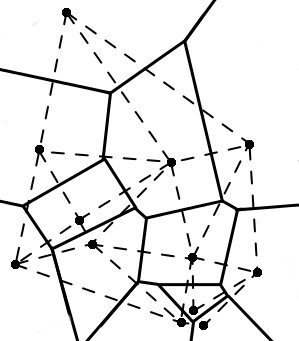
\includegraphics[width=0.5\linewidth]{figs/voronoi}
	\caption{An example Voronoi diagram for objects on a 2-dimensional space.  The black lines correspond to the borders of the Voronoi region, while the dashed lines correspond to the edges of the Delaunay Triangulation.}
	\label{voro-ex}
\end{figure}




The Distributed Greedy Voronoi Heuristic (DGVH) is a fast method for nodes to define their individual Voronoi region (Algorithm \ref{alg:dgvh}). 
This is done by selecting the nearby nodes that would correspond to the points connected to it by a Delaunay triangulation.
The rationale for this heuristic is that, in the majority of cases, the midpoint between two nodes falls on the common boundary of their Voronoi regions.

%In addition, nodes should only have to compute their own Voronoi region, and possibly estimate those of its neighbors. 
%Anything else is a waste of processing power.



\begin{algorithm} % make smaller
	\caption{Distributed Greedy Voronoi Heuristic}
	\label{alg:dgvh}
	\begin{algorithmic}[1]  % the numberis how many lines
		\State Given node $n$ and its list of $candidates$.
		\State Given the minimum $table\_size$
		\State $short\_peers \leftarrow$ empty set that will contain $n$'s one-hop peers
		\State $long\_peers \leftarrow$ empty set that will contain $n$'s two-hop peers    
		\State Sort $candidates$ in ascending order by each node's distance to $n$
		\State Remove the first member of $candidates$ and add it to $short\_peers$
		\ForAll{$c$ in $candidates$}
		\State $m$ is the midpoint between $n$ and $c$
		\If{Any node in $short\_peers$ is closer to $m$ than $n$}
		\State Reject $c$ as a peer
		\Else
		\State Remove $c$ from $candidates$
		\State Add $c$ to $short\_peers$
		\EndIf
		\EndFor
		\While{$|short\_peers| < table\_size$ \textbf{and} $|candidates| >0$}
		\State Remove the first entry $c$ from $candidates$
		\State Add $c$ to $short\_peers$
		\EndWhile
		\State Add $candidates$ to the set of $long\_peers$	
		\If{$|long\_peers| > table\_size^2$}
		\State $long\_peers \leftarrow$ random subset of $long\_peers$ of size $table\_size^2$
		\EndIf
	\end{algorithmic}
\end{algorithm}


During each cycle, nodes exchange their peer lists with a current neighbor and then recalculate their neighbors.  
A node combines their neighbor's peer list with its own to create a list of candidate neighbors.
This combined list is sorted from closest to furthest.
A new peer list is then created starting with the closest candidate.
The node then examines each of the remaining candidates in the sorted list and calculates the midpoint between the node and the candidate.
If any of the nodes in the new peer list are closer to the midpoint than the candidate, the candidate is set aside.  
Otherwise the candidate is added to the new peer list.


DGVH never actually solves for the actual polytopes that describe a node's Voronoi region.
This is unnecessary and prohibitively expensive \cite{raynet}.
Rather, once the heuristic has been run, nodes can determine whether a given point would fall in its region.

Nodes do this by calculating the distance of the given point to itself and other nodes it knows about.
The point falls into a particular node's Voronoi region if it is the node to which it has the shortest distance.
This process continues recursively until a node determines that itself to be the closest node to the point.
Thus, a node defines its Voronoi region by keeping a list of the peers that bound it.



\subsubsection{Algorithm Analysis}

DVGH is very efficient in terms of both space and time.
Suppose a node $n$ is creating its short peer list from $k$ candidates in an overlay network of $N$ nodes. 
The candidates must be sorted, which takes $O(k\cdot\lg(k))$ operations.  
Node $n$ must then compute the midpoint between itself and each of the $k$ candidates.  
Node $n$ then compares distances to the midpoints between itself and all the candidates.  
This results in a cost of 

\[ k\cdot\lg(k) + k \text{ midpoints}  + k^{2} \text{ distances} \]


Since $k$ is  bounded by $\Theta(\frac{\log N}{\log \log N} )$ \cite{bern1991expected} (the expected maximum degree of a node), we can translate the above to

\[O(\frac{\log^{2} N}{\log^{2} \log N} )\]

In the vast majority of cases, the number of peers is equal to the minimum size of \textit{Short Peers}. 
This yields $k=(3d+1)^{2}+3d+1$ in the expected case, where the lower bound and expected complexities are $\Omega(1)$.


%\subsection*{Peerlist and Topology}
%Like CAN \cite{can}, VHash tracks only neighbors for it's peers.
%We enforce a lower limit on the size of the peerlist to avoid nodes being 


%\subsection*{Joining}


%\subsection*{Fault Tolerance}


\section{Summary}
%TODO:  Add a paragraph here
% % % table
% Perhaps geometries should be included?
% be sure to include join and leave costs.

\begin{table}[h]
	\small
	\centering
	\begin{tabularx}{\textwidth}{ |X|X|X|X|X| }
		\hline
		% Add join leave cost, avgerages and maxs
		DHT & Routing Table Size & Lookup Time & Join/Leave & Comments \\ \hline  
		
		Chord \cite{chord} & $O(\log n)$, maximum $m +2s$ & $O(\log n)$, avg $\frac{1}{2} \log n)$  &  $<O(\log n^{2})$ total messages& $m$  = keysize in bits, $s$ is neighbors in 1 direction  \\ \hline
		
		Kademlia \cite{kademlia} & $O(\log n)$, maximum $m\ \cdot k$ & $\lceil \log n\rceil) + c$ & $O(\log(n))$& This is without considering optimization   \\ \hline
		CAN \cite{can} & $\Omega(2d)$ & $O(n^{\frac{1}{d}})$, average $\frac{d}{4}\cdot n^{\frac{1}{d}}$ & Affects $O(d)$ nodes & $d$ is the number of dimensions \\ \hline
		
		Plaxton-based DHTs, Pastry \cite{pastry}, Tapestry \cite{tapestry} & $O(\log_{\beta} n)$ & & &  NodeIDs are base $\beta$ numbers \\ \hline
		
        Symphony \cite{symphony}& $2k + 2$&   average $O(\frac{1}{k} \log^{2} n )$ & $O(\log^{2} n)$ messages,  constant $<1$ &  $k \geq 1$, fingers are chosen at random\\ \hline  
		
        ZHT \cite{li2013zht}&   $O(n)$& $O(1)$ &  $O(n)$ & Assumes an extremely low churn \\ \hline
        
        VHash & $\Omega(3d+1) + O((3d+1)^{2})$ & $O(\sqrt[d]{n})$ hops & $3d + 1$ & approximates regions, hops are based least latency\\ \hline
	\end{tabularx}
	\caption{The different ratios and their associated DHTs}
	\label{tab:tradeoffs}
\end{table}

% % % Specific DHTs



